\documentclass[11pt ,a4paper , twoside , openright ]{article}
\usepackage[T1]{fontenc}
\usepackage[utf8]{inputenc}
\usepackage{lmodern}
\usepackage{hyperref}
\usepackage[a4paper,top=3cm,bottom=3cm,left=2.5cm,right=2.5cm]{geometry}
\usepackage[square,numbers]{natbib}
\bibliographystyle{abbrvnat}
\usepackage[italian]{babel}
\usepackage[usenames]{color} 
\usepackage{listings} 
\usepackage{color}
\usepackage{graphicx}
\usepackage[bottom]{footmisc}
\graphicspath{ {./images/} }
\definecolor{mygreen}{rgb}{0,0.6,0}
\definecolor{mygray}{rgb}{0.5,0.5,0.5}
\definecolor{mymauve}{rgb}{0.58,0,0.82}

\lstset{ 
	backgroundcolor=\color{white}, 
	basicstyle=\footnotesize,
	breakatwhitespace=false, 
	breaklines=true,
	captionpos=b, 
	commentstyle=\color{mygreen}, 
	escapeinside={\%*}{*)}, 
	extendedchars=true, 
	frame=single,
	keepspaces=true, 
	keywordstyle=\color{blue},
	morekeywords={*,...}, 
	numbers=left, 
	numbersep=5pt, 
	numberstyle=\tiny\color{mygray}, 
	rulecolor=\color{black}, 
	showspaces=false, 
	showstringspaces=false, 
	showtabs=false, 
	stepnumber=1, 
	stringstyle=\color{mymauve}, 
	tabsize=2, 
}

\definecolor{darkgray}{rgb}{.4,.4,.4}
\definecolor{purple}{rgb}{0.65, 0.12, 0.82}

\lstdefinelanguage{JavaScript}{
	keywords={typeof, new, true, false, catch, function, return, null, catch, switch, var, if, in, while, do, else, case, break},
	keywordstyle=\color{blue}\bfseries,
	ndkeywords={class, export, boolean, throw, implements, import, this},
	ndkeywordstyle=\color{darkgray}\bfseries,
	identifierstyle=\color{black},
	sensitive=false,
	comment=[l]{//},
	morecomment=[s]{/*}{*/},
	commentstyle=\color{purple}\ttfamily,
	stringstyle=\color{red}\ttfamily,
	morestring=[b]',
	morestring=[b]"
}

\lstset{
	language=JavaScript,
	extendedchars=true,
	basicstyle=\small\ttfamily,
	showstringspaces=false,
	showspaces=false,
	numbers=left,
	numberstyle=\scriptsize,
	numbersep=9pt,
	tabsize=2,
	breaklines=true,
	showtabs=false,
	captionpos=b
}

\author{
	Daniele Rigon - 857319 \\
}

\begin{document}
\title{Tesi - Service Workers}
\maketitle

\tableofcontents
\pagebreak

\section{Overview}
Un ServiceWorker è uno script Javascript che utilizza le Promises per poter eseguire operazioni in modalità asincrona nel browser, avviate in background separato dalla pagina; pertanto non possono modificarne gli elementi del DOM come i normali script ma può comunicare con essi mediante “messaggi”.
Un ServiceWorker si trova tra la nostra applicazione Web e la rete e, come un server proxy, può intercettare tutte le richieste a pagine web e file statici e rispondere secondo politiche che siamo noi stessi a decidere.
I ServiceWorker sono pensati per consentire la creazione di esperienze offline efficaci, intercettare le richieste di rete e intraprendere azioni appropriate in base al fatto che la rete sia disponibile o meno e aggiornare le risorse che risiedono sul server, oltre a consentire l'accesso alle notifiche push e alle API di sincronizzazione in background.
È il browser che in qualsiasi momento deciderà se il ServiceWorker dovrebbe essere o meno in esecuzione così da risparmiare risorse, specialmente sui dispositivi mobili. Per questo può essere che se non facciamo alcuna richiesta HTTP per un certo periodo di tempo o non riceviamo alcuna notifica per un po' è possibile che il browser spenga il Service Worker. Se attiviamo una richiesta HTTP che deve essere gestita dal ServiceWorker il browser la attiverà di nuovo, nel caso in cui non fosse ancora in esecuzione. 

\subsection{Impostare i service worker}
Molte funzionalità dei Service Worker oggi sono abilitate di default, ma nel caso non lo fossero bisogna abilitarle nel browser:
\begin{itemize}
	\item Firefox: su \url{about:config} impostare dom.serviceWorkers.enabled su true, riavvia il browser;
	\item Chrome : su \url{chrome://flags} accendere  experimental-web-platform-features, riavvia browser;
	\item Opera : su \url{opera://flags} attivare Support for ServiceWorker, riavvia il browser;
	\item Microsoft Edge : su \url{about:flags} spuntare  Enable service workers, riavvia il browser.
\end{itemize}

\subsection{Architettura di base}
Per quanto riguarda i ServiceWorker generalmente vengono eseguiti questi passaggi per l'impostazione di base:
\begin{itemize}
	\item L'URL del ServiceWorker viene recuperato e registrato tramite serviceWorkerContainer.register();
	\item In caso di esito positivo il ServiceWorker viene eseguito in un ServiceWorkerGlobalScope, ovvero un tipo speciale di ServiceContext che scappa dal thread di esecuzione dello script principale senza accesso DOM. Il ServiceWorker ora è pronto per elaborare gli eventi;
	\item L'installazione del ServiceWorker viene tentata quando si accede successivamente alle pagine: un evento di installazione è sempre il primo inviato a un ServiceWorker;
	\item Quando il ServiceWorker è considerato installato il passo successivo è l'attivazione, quindi quando il ServiceWorker è installato riceve un evento di attivazione.
\end{itemize}
\begin{figure}[h]
	\centering
	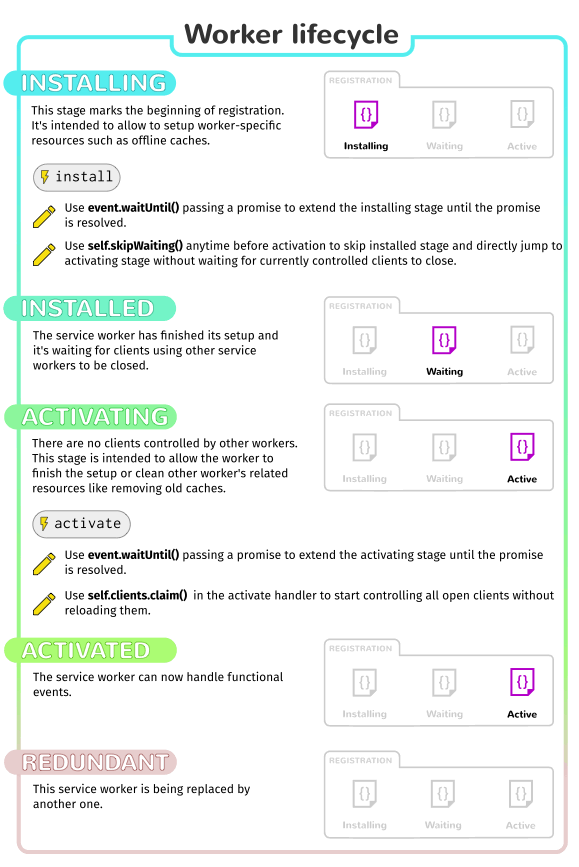
\includegraphics[width=0.6\linewidth]{SwLifecycle}
	\caption{Ciclo di vita del Service Worker}
	\label{fig:Ciclo di vita del Service Worker}
\end{figure}

\subsection{Casi d'uso}
I Service Worker sono destinati anche ad altri usi:
\begin{itemize}
	\item Sincronizzazione dei dati in background;
	\item Risposta a richieste di risorse da altre origini;
	\item Ricezione di aggiornamenti centralizzati a dati costosi da calcolare in modo che più pagine possano utilizzare un set di dati;
	\item Modelli personalizzati basati su determinati pattern URL;
	\item Miglioramenti delle prestazioni, ad esempio prelettura delle risorse che l'utente probabilmente avrà bisogno nel prossimo futuro.
\end{itemize}
Altre specifiche sono utilizzate dal Service Context, ad esempio:
\begin{itemize}
	\item Sincronizzazione in background : avvia un operatore di servizio anche quando nessun utente si trova sul sito, quindi le cache possono essere aggiornate, ecc;
	\item Reagire per inviare messaggi : si può avviare un Service Worker per inviare agli utenti un messaggio per comunicare loro che sono disponibili nuovi contenuti;
	\item Reagendo ad orari e date particolari.
\end{itemize}
\newpage
\section{Ciclo di vita di un Service Worker}
Il ciclo di vita di un service worker è composto da quattro fasi:
\begin{itemize}
\item Registrazione: il service worker viene scaricato dal browser, analizzato ed eseguito;
\item Installazione: il service worker viene installato;
\item Attivazione: il service worker è pronto ed è in grado di poter controllare gli eventi generati dal client;
\item Fetch: evento generato dal client. Il service worker è in grado di intercettare le richieste e rispondere secondo le opportune strategie di caching. 
\end{itemize}

\subsection{Registrazione}

Come prima cosa bisogna comunicare al browser l’esistenza di un ServiceWorker all’interno del sito web. Un ServiceWorker viene prima registrato utilizzando il metodo ServiceWorker.register() e per farlo basta inserire su tutte le pagine del sito uno script come il seguente:
\begin{lstlisting}
if ('serviceWorker' in navigator) { 
	// Path che contiene il service worker navigator.serviceWorker.register('/service-worker.js').then(function(registration) { 			 		
	console.log('Service worker installato correttamente, ecco lo scope:', registration.scope); }).catch(function(error) { 
			console.log('Installazione service worker fallita:', error); 
		});
}
\end{lstlisting}
Il codice inizia controllando il supporto da parte del browser verificando la presenza di navigator.serviceWorker. Se supportato, il ServiceWorker viene registrato per mezzo di navigator.serviceWorker.register che restituisce un oggetto Promise il quale si risolve con successo a registrazione avvenuta correttamente.
service-worker.js è il file Javascript residente nella root del sito web e che contiene il codice del service worker, il cui codice è:
\begin{lstlisting}
// Evento install
self.addEventListener('install', event => { // Codice da eseguire su installazione console.log("Service Worker Installato");
});
// Evento activate
self.addEventListener('activate', event => { // Codice da eseguire su attivazione console.log("Service Worker Attivo");
});
// Evento fetch
self.addEventListener('fetch', event => { // Codice da eseguire su fetch di risorse console.log("Richiesta URL: "+event.request.url);
});
\end{lstlisting}

In questo modo viene registrato un ServiceWorker il quale viene semplicemente installato e ad ogni richiesta stampa in console un messaggio con la URL che il browser tenta di scaricare dal server web. Per controllare il caricamento di un Service Worker il codice di questo deve essere eseguito al di fuori delle normali pagine.

Possono esserci diversi motivi per cui il Service Worker non si registra:
\begin{itemize}
	\item Non si sta eseguendo l'applicazione tramite HTTPS;
	\item Il path del Service Worker non è scritto correttamente: deve essere scritto in relazione all'origine, non alla directory radice dell'app;
	\item Il Service Worker a cui ci si riferisce ha un'origine diversa da quella della tua app.
\end{itemize}

\subsection{Installazione}
Il ServiceWorker viene scaricato immediatamente quando un utente accede per la prima volta a un sito, o una pagina, controllata dal ServiceWorker, e sarà poi scaricato periodicamente ogni tot periodo di tempo.

L'installazione viene tentata quando il file nuovo che è stato scaricato risulta diverso da un ServiceWorker esistente, o risulta essere diverso dal primo ServiceWorker rilevato per quella pagina/sito. Se è la prima volta che un ServiceWorker viene reso disponibile viene tentata l'installazione e, dopo un'installazione corretta, viene attivato. Se è disponibile un ServiceWorker esistente la nuova versione viene installata in background, ma non ancora attivata; si attiva solo quando non ci sono più pagine caricate che stanno ancora utilizzando il vecchio ServiceWorker. Non appena non ci sono più pagine da caricare il nuovo ServiceWorker si attiva.

Conseguentemente all’installazione viene richiamato l’evento install: tale evento consente di effettuare il precaching, ovvero inserire in cache pagine e file statici del sito web prima di intercettarne le richieste. Per farlo occorre utilizzare gli oggetti Promise event e cache come segue:
\begin{lstlisting}
	'use strict';
	// Array di configurazione del service worker
	var config = {
	version: 'versionesw1::',
	// Risorse da inserire in cache immediatamente - Precaching
	staticCacheItems: [ '/wp-includes/js/jquery/jquery.js', '/wp-content/themes/miotema/logo.png', '/wp-content/themes/miotema/fonts/opensans.woff', '/wp-content/themes/miotema/fonts/fontawesome-webfont.woff2',
	],
	};
	// Funzione che restituisce una stringa da utilizzare come chiave per la cache
	function cacheName (key, opts) { return `${opts.version}${key}`;
	}
	// Evento install
	self.addEventListener('install', event => { event.waitUntil( // Inserisco in cache le URL configurate in config.staticCacheItems caches.open( cacheName('static', config) ).then(cache => cache.addAll(config.staticCacheItems)) // self.skipWaiting() evita l'attesa, il che significa che il service worker si attivera immediatamente non appena conclusa l'installazione .then( () => self.skipWaiting() ) ); console.log("Service Worker Installato");
	});
\end{lstlisting}
Se si decidesse di aggiungere/eliminare nuove risorse da inserire in cache bisognerà avere l’accortezza di cambiare il nome della versione del ServiceWorker ed eliminare dalla cache le risorse già presenti.
Una cosa molto importante da sapere è che le risorse da inserire in cache in fase di precaching devono esistere realmente sul server web altrimenti il ServiceWorker genererà un errore fatale e l’installazione non andrà a buon fine. 
Il metodo skipWaiting() consente al ServiceWorker di passare allo stato di attivazione ad installazione conclusa e quindi essere subito operativo.

\subsection{Attivazione}
Una volta installato il ServiceWorker passa nello stato di attivazione. Se la pagina al momento è controllata da un altro ServiceWorker quello attuale passa in uno stato di attesa per poi diventare operativo al prossimo caricamento di pagina quando il vecchio ServiceWorker viene sostituito.
Questo per essere sicuri che solo un ServiceWorker (o una sola versione di ServiceWorker) per volta possa essere eseguito nello stesso contesto.
A ServiceWorker attivato viene richiamato l’evento activate, ovvero l'evento per svuotare la cache obsoleta dell’eventuale precedente versione di ServiceWorker. Dopodiché il ServiceWorker sarà in grado di effettuare il fetching di risorse o di restare in attesa di altri eventi.
Di default il nuovo ServiceWorker diventa operativo al refresh della pagina o dopo aver richiamato il metodo clients.claim(); fino a quel momento le eventuali richieste non saranno intercettate. 

\subsection{Fetch}
Grazie all’evento fetch il ServiceWorker potrà agire da proxy tra l’applicazione web e la rete.
Il ServiceWorker intercetterà ogni richiesta HTTP del browser e sarà in grado di rispondere a quest’ultimo prendendo la risorsa dalla cache piuttosto che scaricarla dalla rete.
Grazie all’evento fetch il ServiceWorker diventa un vero e proprio strumento per migliorare le performance di caricamento di un sito web.

\subsection{Aggiornare il Service Worker}
Se il ServiceWorker è già stato installato ma una nuova versione è disponibile per l'aggiornamento o il caricamento della pagina, la nuova versione viene installata in background ma non sarà ancora attivata. Si attiva solo quando non ci sono più pagine caricate che stanno ancora utilizzando il vecchio servizio. Non appena non ci sono più pagine di questo tipo ancora caricate, il nuovo ServiceWorker si attiverà.

Si dovrà aggiornare il listener install di eventi nel nuovo Service Worker, similmente a questo:
\begin{lstlisting}
self.addEventListener('install', function(event) {
	event.waitUntil(
		caches.open('v2').then(function(cache) {
			return cache.addAll([
				'/sw-test/',
				'/sw-test/index.html',
				'/sw-test/style.css',
				'/sw-test/app.js',
				'/sw-test/image-list.js',
								
				// include other new resources for the new version...
			]);
		})
	);
});
\end{lstlisting}
Mentre accade questo è ancora la versione precedente (v1) quella responsabile per i recuperi, mentre la nuova versione (v2) si sta installando in background.
Quando nessuna pagina sta utilizzando la versione corrente, il nuovo operatore si attiva e diventa responsabile dei recuperi.

\subsection{Disintallare il Service Worker}

Rimuovere/disinstallare un ServiceWorker è un’operazione semplice. È possibile eseguirla manualmente dal proprio browser oppure inserendo un semplice script al posto di quello di registrazione del service worker:

\begin{lstlisting}
	navigator.serviceWorker.getRegistrations().then(function(registrations) { 		
		for(let registration of registrations) { 
			registration.unregister() 
		}
	})
\end{lstlisting}

Naturalmente è necessario che la pagina contenente il codice di disinstallazione venga visitata dal browser, oppure è possibile rimuovere il ServiceWorker manualmente tramite DevTools.
\newpage
\section{Strategie di caching}
Diverse sono le strategie che possono essere adottate per migliorare le performance di un sito web mediante i service worker. A seconda del sito e del contesto è possibile adottare una strategia piuttosto che l’altra.
È importante sottolineare che il ServiceWorker non utilizza cache a meno che non siamo noi a dirlo, quindi di default il comportamento nella fase di fetch delle risorse sarà quello nativo del browser.
Di seguito l’elenco completo delle strategie con esempi di codice di implementazione. 
\subsection{Network first}
Questa strategia mira ad avere un contenuto sempre fresco scaricandolo dalla rete, fornendo la copia in cache solo in caso di problemi di connettività (ad esempio in caso di connessione offline).
\begin{lstlisting}
self.addEventListener('fetch', function(event) { 
		event.respondWith(fetch(event.request).catch(function() { 
			return caches.match(event.request); 
		}) 
	);
});
\end{lstlisting}
Una modifica interessante in questo caso potrebbe essere quella di aggiornare la copia in cache quando la risorsa viene scaricata dalla rete, cosicché in caso di errori di connessione viene restituita la copia più giovane.
\begin{lstlisting}
self.addEventListener('fetch', function(event){ 
		event.respondWith(fetch(event.request).then(function(response) { 		
			cache.put(event.request, response.clone()); 
			return response; 
		}).catch(function() { 
			return caches.match(event.request); 
		}) 
	);
});
\end{lstlisting}
\begin{figure}[h]
	\centering
	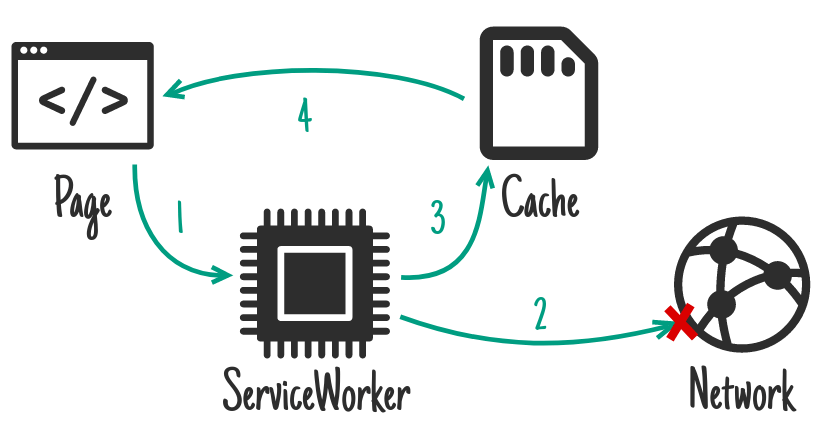
\includegraphics[width=1\linewidth]{Strategia1}
	\caption{Network first}
	\label{fig: Network first}
\end{figure}
\pagebreak
\subsection{Cache first}
Chiamata anche cache, falling back to network, questa strategia verifica se la risorsa è disponibile in cache. Se così fosse viene restituita la copia in cache. In caso contrario la risorsa viene scaricata dalla rete.
\begin{lstlisting}
self.addEventListener('fetch', function(event) {
	event.respondWith(
		caches.match(event.request).then(function(response) {
			return response || fetch(event.request);
		})
	);
});
\end{lstlisting}
\begin{figure}[h]
	\centering
	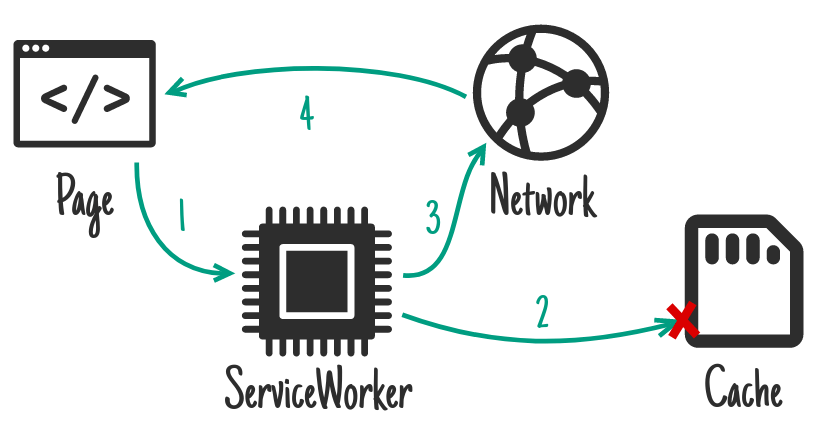
\includegraphics[width=1\linewidth]{Strategia2}
	\caption{Cache First}
	\label{fig: Cache First}
\end{figure}
\pagebreak
\subsection{Network only}
È la strategia più banale in quanto viene simulato il normale comportamento del browser, ovvero scaricare le risorse direttamente dalla rete.

Per applicare  questa strategia basta non inserire alcuna riga di codice all’interno dell’evento fetch:
\begin{lstlisting}
self.addEventListener('fetch', function(event) {});
\end{lstlisting}
o al limite inserire semplicemente la seguente riga:
\begin{lstlisting}
self.addEventListener('fetch', function(event) {
	event.respondWith(fetch(event.request));
});
\end{lstlisting}
\begin{figure}[h]
	\centering
	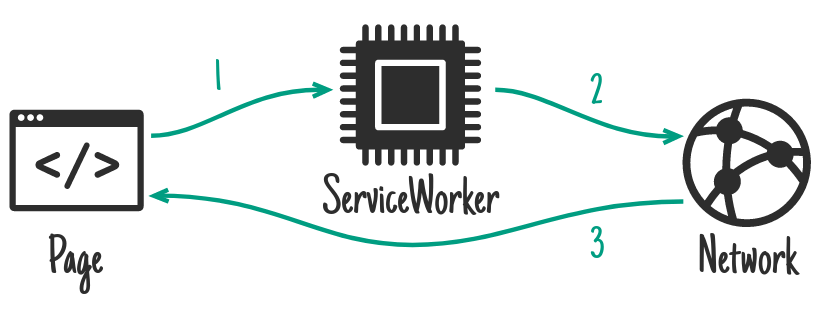
\includegraphics[width=1\linewidth]{Strategia3}
	\caption{Network only}
	\label{fig: Network only}
\end{figure}
\pagebreak
\subsection{Cache only}
Esattamente opposta alla strategia network only, in questo caso il service worker risponde solo con elementi conservati in cache. In caso di miss la risposta restituita al browser simulerà l’errore di connessione.
\begin{lstlisting}
self.addEventListener('fetch', function(event) {
	event.respondWith(caches.match(event.request));
});
\end{lstlisting}
\begin{figure}[h]
	\centering
	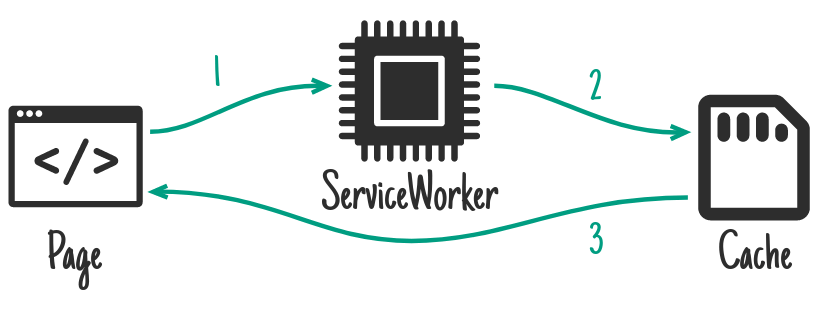
\includegraphics[width=1\linewidth]{Strategia4}
	\caption{Cache Only}
	\label{fig: Cache Only}
\end{figure}
\pagebreak
\subsection{Fastest}
Questa strategia mira a fornire all’utente la risposta più veloce. Il ServiceWorker avvia contemporaneamente una richiesta in cache ed una in rete. La prima che risponde verrà restituita all’utente.
Questa soluzione può essere l’ideale per quei dispositivi con vecchi hard drive dove la lettura da disco può addirittura rivelarsi più lenta del fetch dalla rete. Per i dispositivi moderni è meglio utilizzare la strategia cache then network.
Siccome il ServiceWorker può ritornare un solo Promise, occorre realizzare una funzione a cui passare un array di oggetti Promise, in questo caso cache e fetch, e risolverli quasi contemporaneamente ritornando quello che si risolve per primo.
\begin{lstlisting}
function promiseAny(promises) { 
	return new Promise((resolve, reject) => { 
		promises = promises.map(p => Promise.resolve(p)); 
		promises.forEach(p => p.then(resolve)); 
		promises.reduce((a, b) => a.catch(() => b)).catch(() => reject(Error("All failed"))); 
	});
};
self.addEventListener('fetch', function(event) { 
	event.respondWith( promiseAny([caches.match(event.request), fetch(event.request)]) );
});
\end{lstlisting}
\begin{figure}[h]
	\centering
	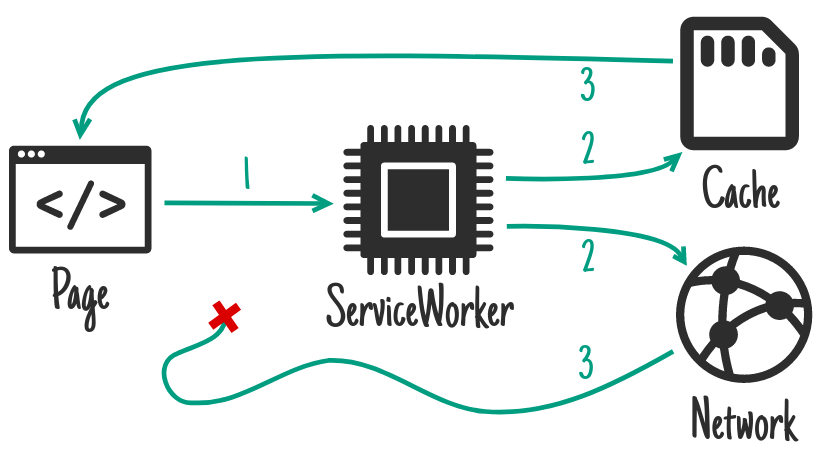
\includegraphics[width=1\linewidth]{Strategia5}
	\caption{Fastest}
	\label{fig: Fastest}
\end{figure}
\pagebreak
\subsection{Cache then network}
Questa strategia mira a fornire il contenuto dalla cache per una risposta molto rapida. Dopodiché in parallelo si avvia una richiesta in rete per scaricare una copia aggiornata della risorsa e sostituirla con quella in cache. La risorsa ricevuta dalla rete viene poi sostituita con quella presente sulla pagina.
Per ottenere questo obiettivo occorre avere sia codice lato pagina che lato ServiceWorker. Questo perché il ServiceWorker deve rispondere subito e non può attendere il completamento di un secondo task senza rallentare l’intera operazione.
Per ottenere qualcosa di analogo usando il solo ServiceWorker occorre utilizzare postMessage affinché la pagina comunichi al service worker la risorsa da interpellare con un secondo fetch, sia esso dalla cache o dalla rete. La complessità rimane uguale ma molto utile in caso si utilizzi il service worker per fare page caching.

\begin{figure}[h]
	\centering
	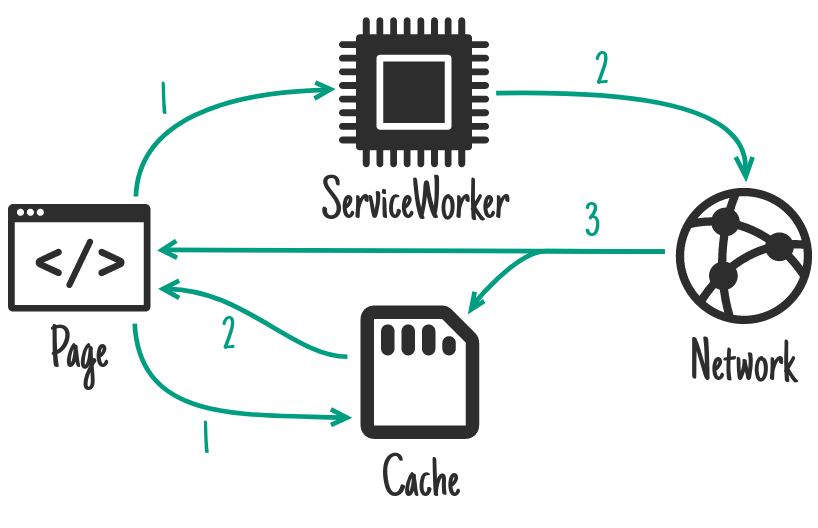
\includegraphics[width=1\linewidth]{Strategia6}
	\caption{Cache then Network}
	\label{fig: Cache then Network}
\end{figure}
\newpage
\section{Rischi e sicurezza}
Come già detto i Service Worker operano solo in contesti protetti, ma questo non vuol dire che l'ambiente sia sicuro al 100\% in quanto un ServiceWorker ha la possibilità di importare script da qualsiasi altra origine tramite la chiamata a importScripts, aumentando la capacità di un attaccante XSS di inserire il proprio codice javascript all'interno della pagina, potendo cosi rubare informazioni dell'utente, ad esempio all'inserimento di username e password in una data pagina e portarle fuori. La registrazione dei Service Worker specifica che essi devono essere eseguiti nella stessa origine dei loro chiamanti; il confronto dell'origine è una corrispondenza col prefisso più lungo degli URL serializzati compreso il percorso, quindi ad esempio https://example.com è differente da https://example.com.evil.com. Quindi un attaccante può effettivamente registrare un Service Worker malevolo. Per mitigare questo rischio il browser richiede che l'URL di registrazione del Service Worker provenga dall'origine stessa; quindi per registrare un Service Worker malevolo attraverso un attacco XSS l'utente malintenzionato ha bisogno di ospitare i propri script sul server.
\\
Un possibile scenario potrebbe essere questo: se la pagina ha una vulnerabilità XSS ha anche un endpoint JSONP \footnote{Utilizzato per richiedere dati da un server che risiede in un dominio diverso da quello del client; consente la condivisione dei dati aggirando la politica della stessa origine} e l'utente malintenzionato potrebbe utilizzarlo per:
\begin{itemize}
	\item bypassare CSP\footnote{Cryptographic Service Provider, libreria software sviluppata da Microsoft};
	\item registrare un Service Worker; 
	\item chiamare importScripts per importare uno script malevolo da terze parti.
\end{itemize}
In una situazione XSS del genere il limite della direttiva cache di 24 ore garantisce che un Service Worker malevolo o compromesso sopravviverà a un massimo di 24 ore, o meno in base a come è impostato il sito. Una possibile mitigazione del problema potrebbe essere accorciare la vita dei Service Worker, ovviamente in modo ragionevole altrimenti non sarebbero sfruttate le potenzialità.
\\
Inoltre un Service Worker potrebbe non essere usato solamente per il caching, migliorando i tempi di risposta dell'applicazione o del sito, ma potrebbe anche essere usato per intercettare messaggi, modificandoli e restituendoli errati (similmente a man-in-the-middle).


- Pro: vedere se i SW possono migliorare la sicurezza di una pagina, senza essere usati solo per fare caching.
\newpage
\section{Esempio di attacco}
Supponiamo di avere questa pagina HTML che carica uno script per l'installazione di un Service Worker, pensando sia sicuro.
\lstinputlisting{../../ServiceWorker/AttaccoXSS/index.html}
Il file script.js sarà il seguente:
\lstinputlisting{../../ServiceWorker/AttaccoXSS/script.js}
Mentre hack.js, che intercetta ogni richiesta, sarà questo:
\lstinputlisting{../../ServiceWorker/AttaccoXSS/hack.js}
Infine il file che installerà il Service Worker malevolo sarà questo:
\lstinputlisting{../../ServiceWorker/AttaccoXSS/install.js}
Ogni richiesta che verrà fatta sarà intercettata dal Service Worker (in questo caso uscirà il messaggio "Intercepted" nella pagina web) fino a che non sarà disinstallato e non verrà cancellata la cache.
\newpage
\section{Compatibilità web}
\subsection{Desktop}
\begin{figure}[h]
	\centering
	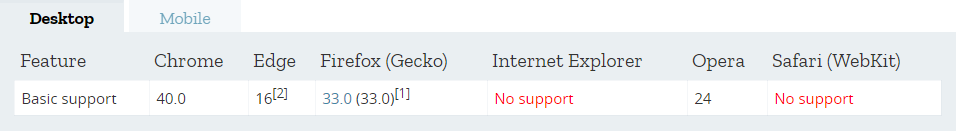
\includegraphics[width=1\linewidth]{CompWeb}
	\caption{Compatibilità web}
	\label{fig:Compatibilità web}
\end{figure}
\subsection{Mobile}
\begin{figure}[h]
	\centering
	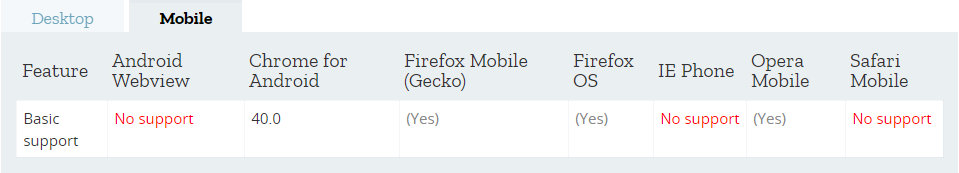
\includegraphics[width=1\linewidth]{CompMobile}
	\caption{Compatibilità mobile}
	\label{fig:Compatibilità mobile}
\end{figure}
\newpage
\section{Conclusioni}
Se realizzati per fare caching i Service Worker possono rendere la navigazione del sito web o dell'applicazione molto più veloce, senza rendere necessarie modifiche al sito o all'applicazione per raggiungere questo scopo. 
Purtroppo sono uno potente strumento anche per scopi malevoli, come illustrato al punto 4.
\newpage
\listoffigures
\newpage
\begin{thebibliography}{99}
	\bibitem{}
	Angular University (2018),
	\emph{Angular Service Worker - Step-By-Step Guide for turning your Application into a PWA},
	\url{https://blog.angular-university.io/angular-service-worker/}
	
	\bibitem{}
	Angular University (),
	\emph{Service Workers - Practical Guided Introduction (several examples)},
	\url{https://blog.angular-university.io/service-workers/}
	
	\bibitem{}
	formatkaka, mfuji09, Jakubem, MichelleKwa12, Adrianjewell91, KateSturmey, tocretpa, danielpox, jpmedley, chrisdavidmills, akshayjai1, dchest, Sebastianz, neonstalwart, jaffathecake, mouki, Sheppy, Zanadar, fbender, DavidWalsh, fscholz, Heydon, teoli, rassoodock, Meggin (2018),
	\emph{Service Worker API},
	\url{https://developer.mozilla.org/en-US/docs/Web/API/Service_Worker_API}
	
	\bibitem{}
	Throne3d, SphinxKnight, jcsahnwaldt, zekrom-vale, fscholz, arvindpdmn, Jiang-Xuan, wbamberg, schalkneethling, b2397, ramsunvtech, Jedipedia, khaled-hossain-code, mzur, anpa, armujahid, zeevmoney, Vectaio, parambirs, JonathanPool, rwaldron, 6112, kushdilip, thenable, hweeks, Jib, rousan, destin.moulton, Soupedenuit, teoli, ZeroUnderscoreOu, stephaniehobson, psl646, fbergr, atpollmann, kberov, jdsjs, booc0mtaco, programmer5000, otherrealm, kdex, CaemU, Granjow, david-mark, abeltanjq, fredmarques, torazaburo, halfzebra, natoen, tarungarg546, vladan1, igniteram, akshatkedia, nathanh, drostie, mamal, fearlessfool, MiLeung, PeteDevoy, RuiBottoFigueira, JonathanWatt, benjamingr, peter.kehl, ole, jacksonrayhamilton, arai, jmrog, jmsbrr, hltbra, jordanluyke, Sheppy, deisner, kamoroso94, dbruant, mdvorak, kristopolous@yahoo.com, pasqLisena, dstorey, bryanrsmith, nalindak, mattclaw, bitzstein, bgdavidx, Sebastianz, neeraj07rathi, kavitshah8, aochagavia, chrisdavidmills, Goldenyz, jpmedley, hexalys, Callmenorm, vinaygopinath, gaspard, slofurno, Jeremie, fkling42, zbuc, skeller88, miller.augusto, astorije, markg, jucrouzet, Delapouite, Gutworth, realityking, Chudesnov, Account, Fantasyshao, deltab., samvermillion, mnoorenberghe, jsantell, dentuzhik, Irving.Reid, Havvy, hthetiot, wesj, Olafk, DomenicDenicola
	\emph{Promise, Mozilla Developer}
	\url{https://developer.mozilla.org/en-US/docs/Web/JavaScript/Reference/Global_Objects/Promise}
	
	\bibitem{}
	DavidGuan, chrisdavidmills, Deleplace, jwhitlock, simon04, mrmaka, bmihelac, erikadoyle, YoranBrondsema, sideshowbarker, joshua1988, jpmedley, kberov, wbamberg, hl222ih, janx, karolklp, tomayac, maybe, UnJavaScripter, ebidel, JCE, philmander, termosa, franzy1709, stevemao, miguelmota, enguerran, allen.dean, fscholz, Brettz9, jryans, teoli, bhritchie, vrana, rippedspine, adria, Sheppy
	\emph{Using Service Workers, Mozilla Developer},
	\url{https://developer.mozilla.org/en-US/docs/Web/API/Service_Worker_API/Using_Service_Workers}
	
	\bibitem{}
	W3C, Alex Russell, Jungkee Song, Jake Archibald, Marijn Kruisselbrink (2018),
	\emph{Service Workers Nightly},
	\url{https://w3c.github.io/ServiceWorker/}
	
	\bibitem{}
	Mozilla,
	\emph{Service Workers},
	\url{https://serviceworke.rs/}
	
	\bibitem{}
	Google Partners,
	\emph{Tecnologie web avanzate: Service worker},
	\url{https://support.google.com/partners/answer/7336697?hl=it}
	
	\bibitem{}
	Speedy Wordpress,
	\emph{Guida completa ai Service Worker Javascript},
	\url{https://www.speedywordpress.it/guida-completa-ai-service-worker-javascript/}
	
	\bibitem{}
	Matt Gaunt,
	\emph{Service Workers: an Introduction},
	\url{https://developers.google.com/web/fundamentals/primers/service-workers/}
	
	\bibitem{}
	SitePoint,
	\emph{Getting Started with Service Workers},
	\url{https://www.sitepoint.com/getting-started-with-service-workers/}
	
	\bibitem{}
	jakearchibald Github (2017),
	\emph{Service workers explained},
	\url{https://github.com/w3c/ServiceWorker/blob/master/explainer.md}
	
	\bibitem{}
	Lyza Danger Gardner
	\emph{Making A Service Worker: A Case Study}
	\url{https://www.smashingmagazine.com/2016/02/making-a-service-worker/}
	
	\bibitem{}
	Eshun Sharma
	\emph{An Introduction to Service Workers in JavaScript},
	\url{https://codeburst.io/an-introduction-to-service-workers-in-javascript-27d6376460c2}
	
	\bibitem{}
	Nicolas Bevacqua (2015), 
	\emph{Making a Simple Site Work Offline with ServiceWorker},
	\url{https://css-tricks.com/serviceworker-for-offline/}
	
	\bibitem{}
	\emph{Service Worker Security FAQ},
	\url{https://chromium.googlesource.com/chromium/src/+/lkcr/docs/security/service-worker-security-faq.md}
\end{thebibliography}
\end{document}